\section{危险因素辨识与评价}

\subsection{危险因素辨识目的和范围}

根据规范《重大危险源辨识》(GB 18218-2018),所谓重大危险源就是指长期或临时地生产、加工、搬运或贮存危险物质,
且危险物质的数量等于或大于临界量的单元。对于路桥工程施工过程中,对于重大危险源的界定主要包括:
人的危险行为及管理的漏洞、物的不安全的状态、恶劣的环境影响等,由于建筑施工现场的复杂性,工程施工事故可能随时发生,
并可导致人员死亡及伤害、破坏、财产损失,这对于建筑施工工程的整体施工进度已经企业的经济效益都会造成恶劣的影响,
甚至危及企业的发展,因此建筑施工过程中对于重大危险源的辨识、评价和控制,就显得格外重要。

对于重大危险源的辨识,可根据对危险源危险等级的评定方法进行,一般是对施工过程中危险源带来的风险进行评价分析,
根据评价结果又针对性地进行风险控制,从而达到持续改进的目的。常用的风险评价方法有:
作业条件危险性评价法(LEC)、矩阵法、预先危害分析 (PHA)、故障类型及影响分析 (FMEA)、风险概率评价法 (PRA)、危险可操作性研究 (HAZOP)、事故树分析 (ETA) 等等。

\subsection{危险源辨识}
\subsubsection{基坑工程危险源辨识}

\quan{1} 由于未经妥善的土层地质水文勘察而导致的坍塌;

\quan{2} 由于未明确周围既有建筑、地下构筑物、基础平面与周围地下管线的关系而导致的坍塌,触电和其他多重伤害;

\quan{3} 由于深基坑作业人员连续加班、疲劳作业而导致的多重伤害;

\quan{4} 由于基坑降水或围护的抗渗设计未有设计妥善或未按照设计方案施工而导致的坍塌;

\quan{5} 由于夜间作业照明不良而引发的包括物体打击和高处坠落在内的多种伤害;

\quan{6} 由于深基坑未设有临边防护措施而造成的高处坠落和物体打击;

\quan{7} 由于土壤内含有有毒物质而并未提供相应的防护措施而导致的中毒;

\quan{8} 由于水平工作面工作间距不足而造成的包括物体打击,机械伤害和触电在内的多重伤害;

\quan{9} 由于汛期无抗洪措施、冻融期未经特殊处理而导致的坍塌;

\quan{10} 由于施工人员未按设计强度用料或施工导致的坍塌;

\quan{11} 作业人员由于误操作,指挥信号不清或抢工而造成的机械伤害;

\quan{12} 由于桩或桩材料不合规或腐蚀而导致的坍塌或物体打击。

\subsubsection{钢筋工程危险源辨识}

\quan{1} 钢筋加工操作人员未经过相关技术交底和培训,不了解钢筋加工机械的操作方法,导致钢筋加工过程中造成机具伤害;

\quan{2} 钢筋作业人员未取得从业资格证件,无特种作业操作证,在焊接过程中误操作导致触电或者火灾;

\quan{3} 预应力钢筋材料进场未经过检验,导致材料不合格;

\quan{4} 钢筋加工机械未经检验或未按时保养,造成在使用过程中造成触电;

\quan{5} 当使用卷扬机进行冷拉操作时,由于卷扬机固定未有妥善导致被拔出而造成的物体打击;或是卷扬机钢丝绳破损而造成的伤害;

\quan{6} 钢筋切断机锯盘无安全防护导致的机械伤害;

\quan{7} 由于未控制钢筋的冷拉率而造成的的超拉现象,导致机械伤害;

\quan{8} 采用切割机进行切割作业时由于无挡板造成火星飞溅而引起火灾;

\quan{9} 带电操作时未执行“一机一闸一箱一漏”的管理规定而导致触电。

\subsubsection{模板工程危险源辨识}

\quan{1} 由于回填土没压实或压实不到位而造成地基不均匀沉降而导致的模板坍塌;

\quan{2} 由于回填土地基未浇筑硂层或未设置垫板而导致的结构问题或模板坍塌;

\quan{3} 由于立杆、水平杆等支架未按规范搭设而导致的整体支架失稳倒塌;

\quan{4} 由于施工方案与设计方案不符而导致的结构失衡而导致模板或支架倒塌;

\quan{5} 由于构建不齐全而导致的体系坍塌;

\quan{6} 由于模板超载使用,或堆放物过于集中而导致的模板破碎;

\quan{7} 由于违规在模板支架上悬挂起重设备、或是混凝土泵送管搭在模板支架而导致的局部荷载超过设计值而造成模板坍塌;

\quan{8} 高大跨模板搭设是未指定检测方案,或是布置检测点位不足而导致的支撑体系变形,
或是地基不均匀沉降。

\subsubsection{混凝土工程危险源辨识}

\quan{1} 由于运送混凝土时操作人重心失稳或脱把而造成的高处坠落;

\quan{2} 由于运送车道上有杂物而导致的运送推车失稳而造成的高处坠落或物体打击;

\quan{3} 由于运送车道过窄而造成的高处坠落或是物体打击;

\quan{4} 由于泵送混凝土管道架设不规范、不牢靠而导致的机械伤害;

\quan{5} 由于混凝土泵未放置稳妥就开始作业而造成的机械伤害;

\quan{6} 由于作业前未进行试压操作而造成的机械伤害或压力容器爆炸;

\quan{7} 由于乱搭乱接泵送管道或其他工具而造成的储电;

\quan{8} 由于操作工具无接地,无绝缘货物或无漏电保护而造成的触电;

\quan{9} 由于混凝土爆模而导致荷载过于集中而超过最大允许荷载而发生坍塌;

\quan{10} 由于临边洞口未经防护而造成的高处坠落或物体打击。

\subsubsection{脚手架工程危险源辨识}

\quan{1} 由于连墙件未按规定搭设、随意拆除、搭设位置或搭设结构不合理而造成的架体倾倒;

\quan{2} 由于基础发生严重破坏或地基不均匀沉降而造成的架体倾倒;

\quan{3} 由于脚手架设计承载力不足而造成超载而引发的架体倾倒;

\quan{4} 由于脚手架作业成没有铺设妥善脚手板,或者是架体边缘的空隙过大而引发的高处坠落;

\quan{5} 由于作业人员高空抛物而造成的物体打击或是高处坠落;

\quan{6} 脚手架上随意堆放物品而造成的物体打击;

\quan{7} 工人作业未有佩戴防护措施而造成的物体打击或高处坠落。

\subsubsection{吊装作业危险源辨识}

\quan{1} 起重机在运行中对人体造成的挤压或撞击;

\quan{2} 起重机吊钩超载断裂、吊运时钢丝绳从吊钩中滑出;

\quan{3} 吊运中重物坠落造成物体打击,重物从空中落到地面又反弹伤人;

\quan{4} 钢丝绳或麻绳断裂造成重物下落;使用应报废的钢丝绳,使用的吊具吊运超过额定起重量的重物等造成重物下落;

\quan{5} 汽车起重机作业场所地面不平整、支撑不稳定、配重不平衡、重物超过额定起重量而造成起重机倾覆;

\quan{6} 风力过大、违章作业造成起重机倾覆;

\quan{7} 机械传动部分未加防护,造成机械伤害;违章在卷扬机钢丝绳上面通过,运动中的钢丝绳将人挤伤或绊倒;

\quan{8} 载货升降机违章载人;

\quan{9} 人站在起重臂下等危险区域。

\subsubsection{其他危险源辨识}

\quan{1} 由于施工车辆未按照规定走行在内部道路引发的车辆伤害;

\quan{2} 由于作业人员未经培训或未经安全交底而造成的多重伤害;

\quan{3} 由于作业人员在进行动火时未报备项目部,开具动火票而造成的火灾或爆炸;

\quan{4} 由于大型机械作业未有明确的指挥信号而造成的包括物体打击,机械伤害和触电在内的多重伤害;

\quan{5} 雪后未经处理就进场作业而导致的包括车辆伤害和物体打击在内的多重伤害;

\quan{6} 作业工人未有佩戴或未按规定佩戴安全绳而导致的物体打击和高处坠落;

\quan{7} 带电工具未进行绝缘测试就投入使用而引发的触电;

\quan{8} 油漆、涂料和胶水未按规定存放而引起的火灾或中毒;

\quan{9} 由于管理人员违章指挥或指挥失误而引起的多重伤害;

\quan{10} 由于手持机具和金属外壳未进行接地操作而造成的触电;

\quan{11} 由于振捣器工作而产生的震动危害;

\quan{12} 由于易燃易爆物质未经妥善储存而引起的火灾、中毒和窒息、爆炸和压力容器爆炸;

\quan{13} 临边洞口未设置警示标志或未设置防护措施而导致的物体打击或高处坠落;

\quan{14} 高压电未有设置专门的配电箱而引发的火灾或爆炸;

\quan{15} 由于高温,高强度工作,酒后上工等个人因素造成的多重伤害。

\subsection{安全评价}
\subsubsection{评价依据}
\subsubsection{评价目的与评价范围}

(1) 评价目的

安全评价目的是查找、分析和预测工程、系统、生产经营活动中存在的危险、有害因素及可能导致的危险、危害后果和程度,提出合理可行的安全对策措施,
指导危险源监控和事故预防,以达到最低事故率、最少损失和最优的安全投资效益。

\quan{1} 系统地从计划、设计、制造、运行、贮运和维修等全过程进行控制。

\quan{2}  建立使系统安全的最优方案,为决策提供依据。

\quan{3} 为实现安全技术、安全管理的标准化和科学化创造条件。促进企业实现本质安全化。

(2) 评价范围

依据《中华人民共和国新安全生产法》,安全评价所涉及的范围是以下经营范围的企业:

\quan{1} 项目在进行可行性研究时,要进行安全生产条件论证和安全预评价,有非煤矿矿山建设项目;

\quan{2} 生产储存危险化学品(包括使用长输管道输送危险化学品)的建设项目;

\quan{3} 生产、储存烟花爆竹的建设项目;

\quan{4} 军工、公路、水运、轨道交通、电力等行业的国家和省级重点建设项目;还有规定的其他项目。

\subsubsection{基坑坍塌事故故障树法安全分析}

基坑坍塌造成的人员伤亡应发生在“基坑坍塌”和“逃生失败”两种情况下。基坑坍塌事故可能是设计问题、施工过程和方法问题,也可能是现场管理不当。
逃跑的失败可以分为“无法逃脱”和“没有意识到生命危险”。基坑坍塌事故故障树见图。\ref{fig:c3f1};

\begin{figure}[thbp!]
    \centering
    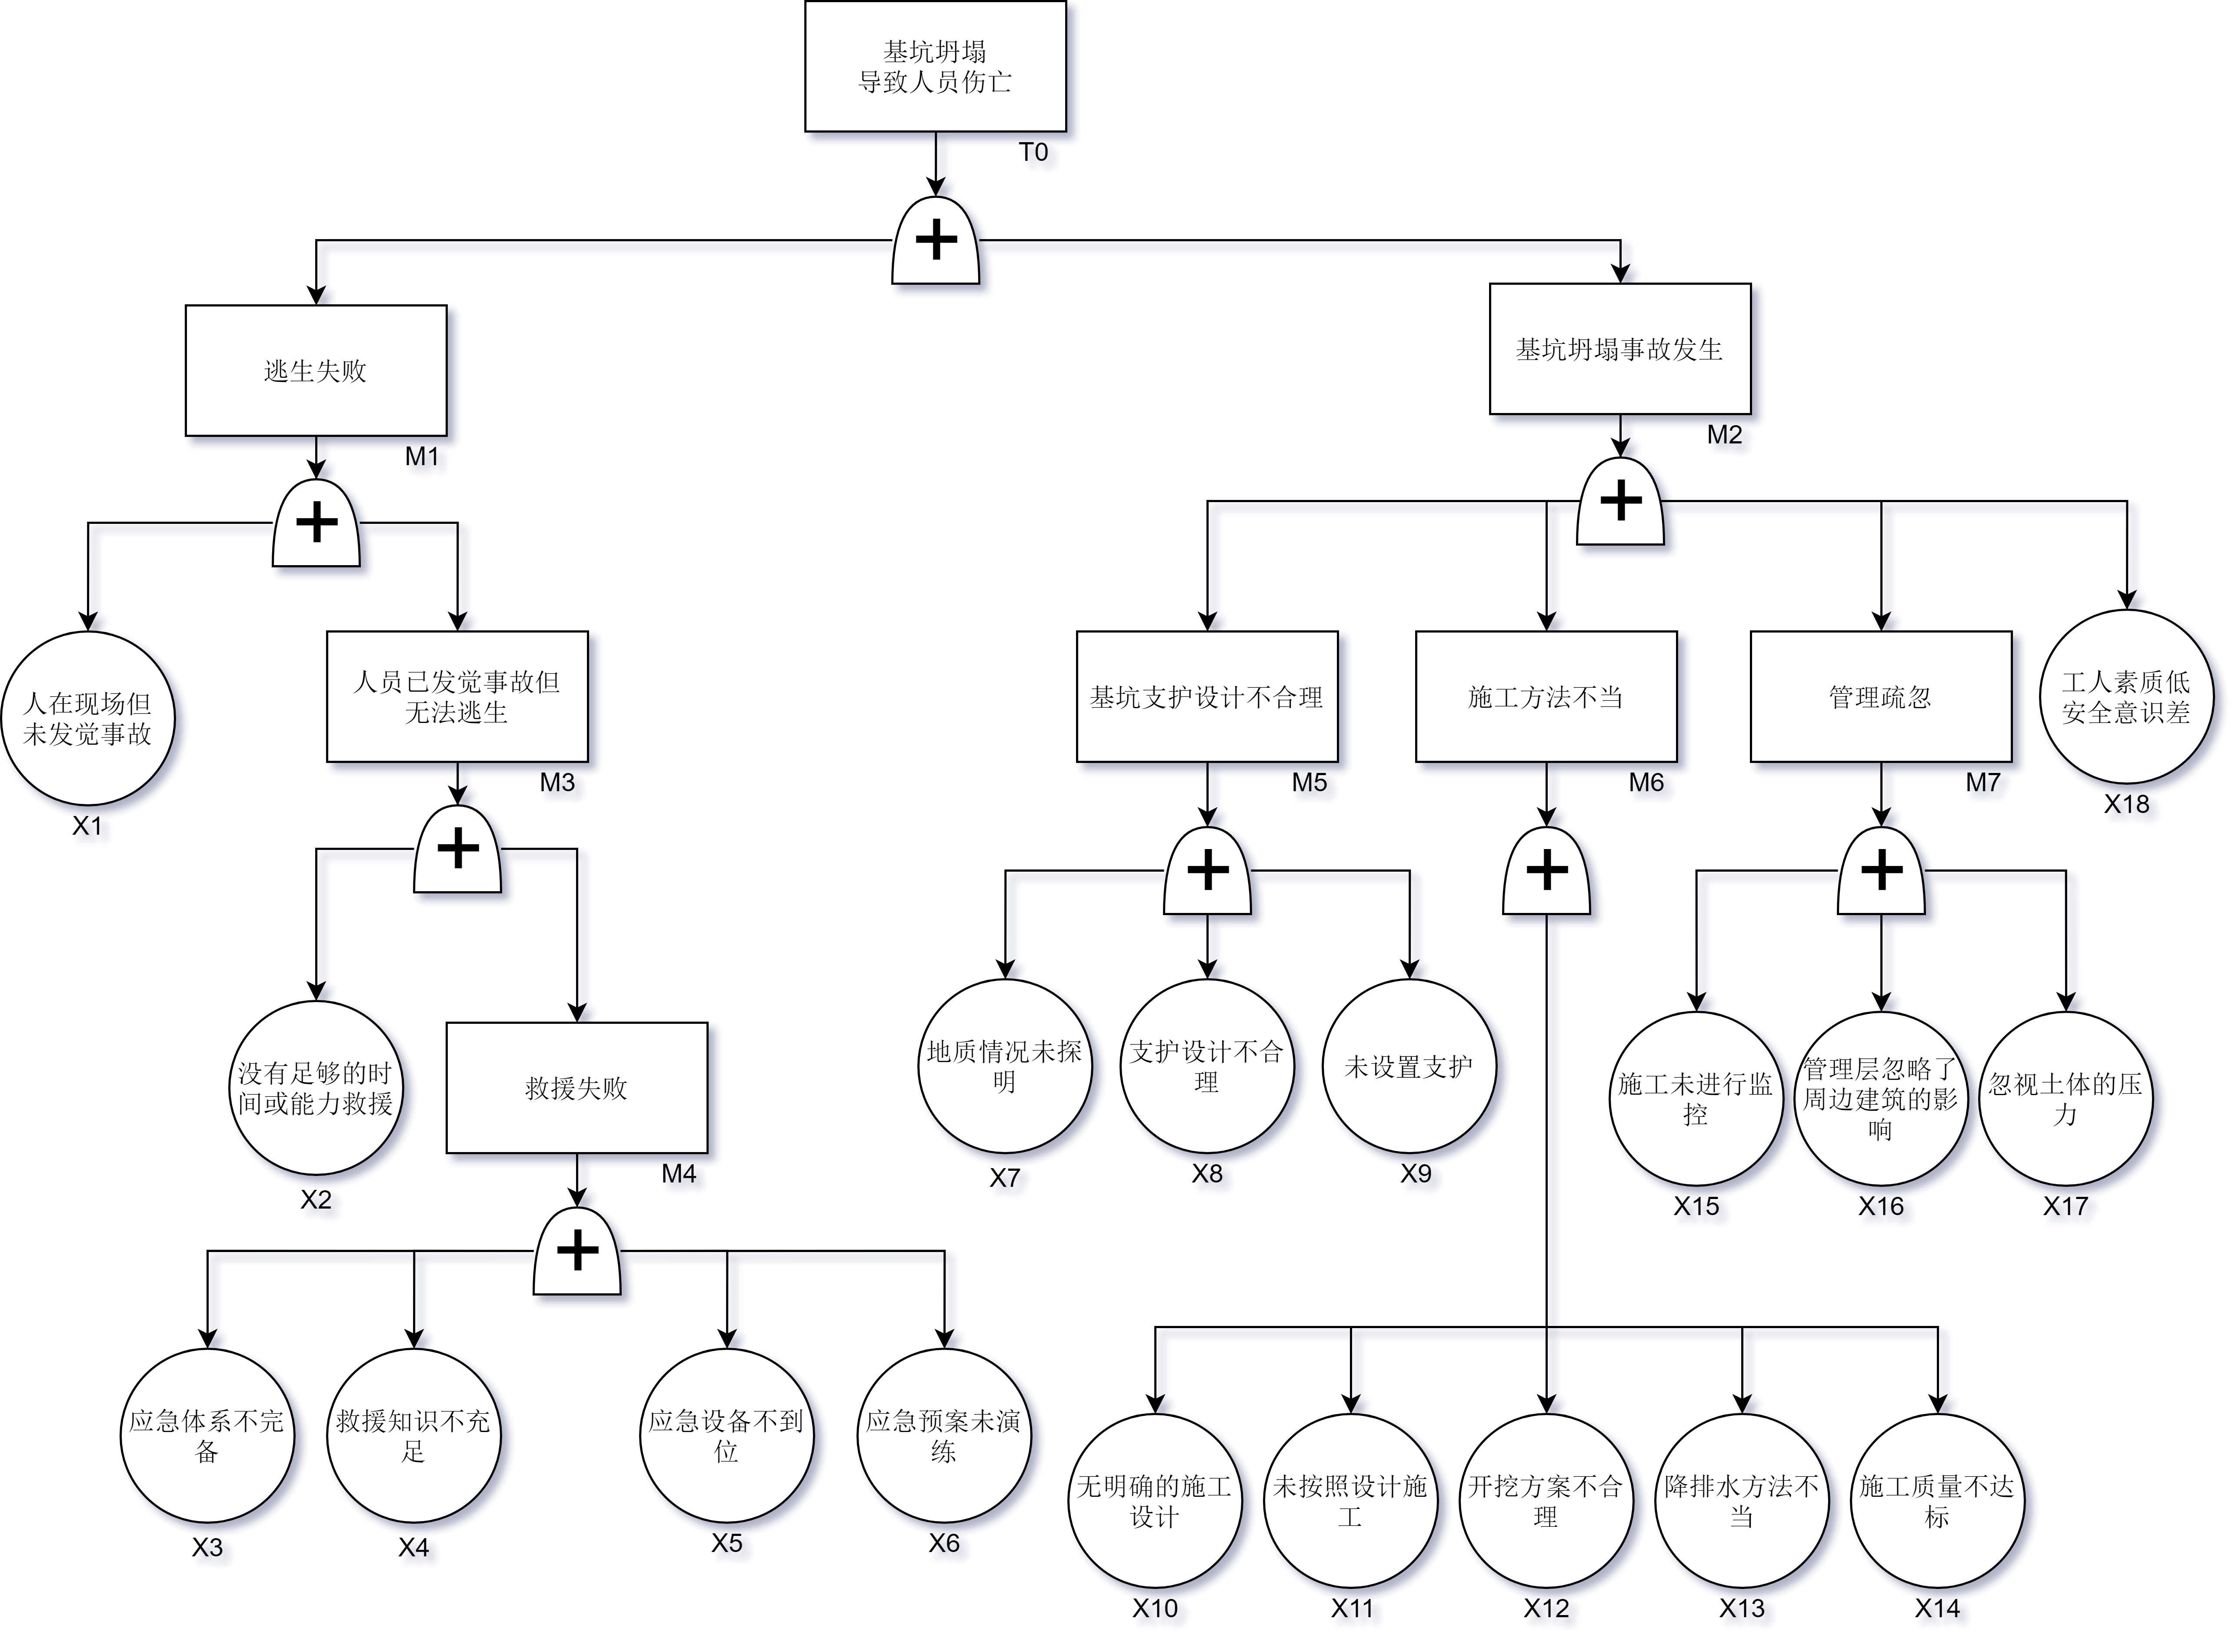
\includegraphics[width=1.0\linewidth]{figure/c3f2.png}
    \caption{基坑坍塌事故树法安全分析}
    \label{fig:c3f1}
\end{figure}

根据图 \ref{fig:c3f1} 列出结构逻辑函数式如下:\\

$T_0=M_1M_2=X_1M_3(M_5+M_6+M_7)=X_1(X_2+M_4)(M_5+M_6+M_7)=X_1[X_2+(X_3+X_4+X_5+X_6)][(X_7+X_8+X_9)+(X_{10}+X_{11}+X_{12}+X_{13}+X_{14})+(X_{15}+X_{16}+X_{17})+X_{18}]$\\

根据布尔代数简化,得到共有 54 组割集,从整理结果可看出,这 54 组都是最小割集。\\

(1) 结果分析\\

\quan{1} 由事故树可知,或门个数多而与门个数少。根据或门定义,只要有任意一个基本事件发生就有输出,而与门表示只有全部基本事件发生时才有输出。

\quan{2} 通过对图 \ref{fig:c3f1} 的定性分析可知,基坑坍塌引起人员伤亡最小割集最多 54 个,最小径集 3 个,即导致基坑坍塌引起人员伤亡的可能性有 54 种,可见基坑坍塌造成人员伤亡是很容易发生的。

\quan{3} 从结构的重要顺序可以看出,在众多的基本原因中,操作人员在事故后未能及时发现安全隐患和危险是最重要的两个因素。其次,设计不到位、施工方法不当、基坑监测不足等因素也导致了事故的发生。\\

(2) 防治办法\\

\quan{1} 安全知识教育、安全技能教育,提高人员安全意识,提高规避风险能力,提高自我防范能力;

\quan{2} 建立和完善应急救援体系,做好应急体系的教育和培训;储备好应急救援设备;开展有针对性的应急救援预案演练,不断提高应急反应能力;

\quan{3} 要加强基坑施工安全技术管理,从设计到施工,制订完善、可行、能操作的安全技术措施,把每一项工作,每一步工序扎扎实实地落实;

\quan{4} 要坚持动态施工,动态设计的原则,一旦发现施工实际情况与原方案不符合,要及时调整施工方案和方法。


\subsubsection{吊装作业事故故障树法安全分析}

造成吊装事故而造成人员伤亡的情况要同时满足“人与起吊物位置不当”和“起吊物坠落”的任意一种事件发生;人与起吊物位置不当的情况有可能是起吊物在人上方经过或人在起吊物下方;
起吊物坠落则有可能在吊钩有缺陷、吊具损坏、司机与工人配合出错等方面中任意发生。
关于吊装作业事故的故障树详见图 \ref{fig:c3f3};

\begin{landscape}
\begin{figure}[thbp!]
    \centering
    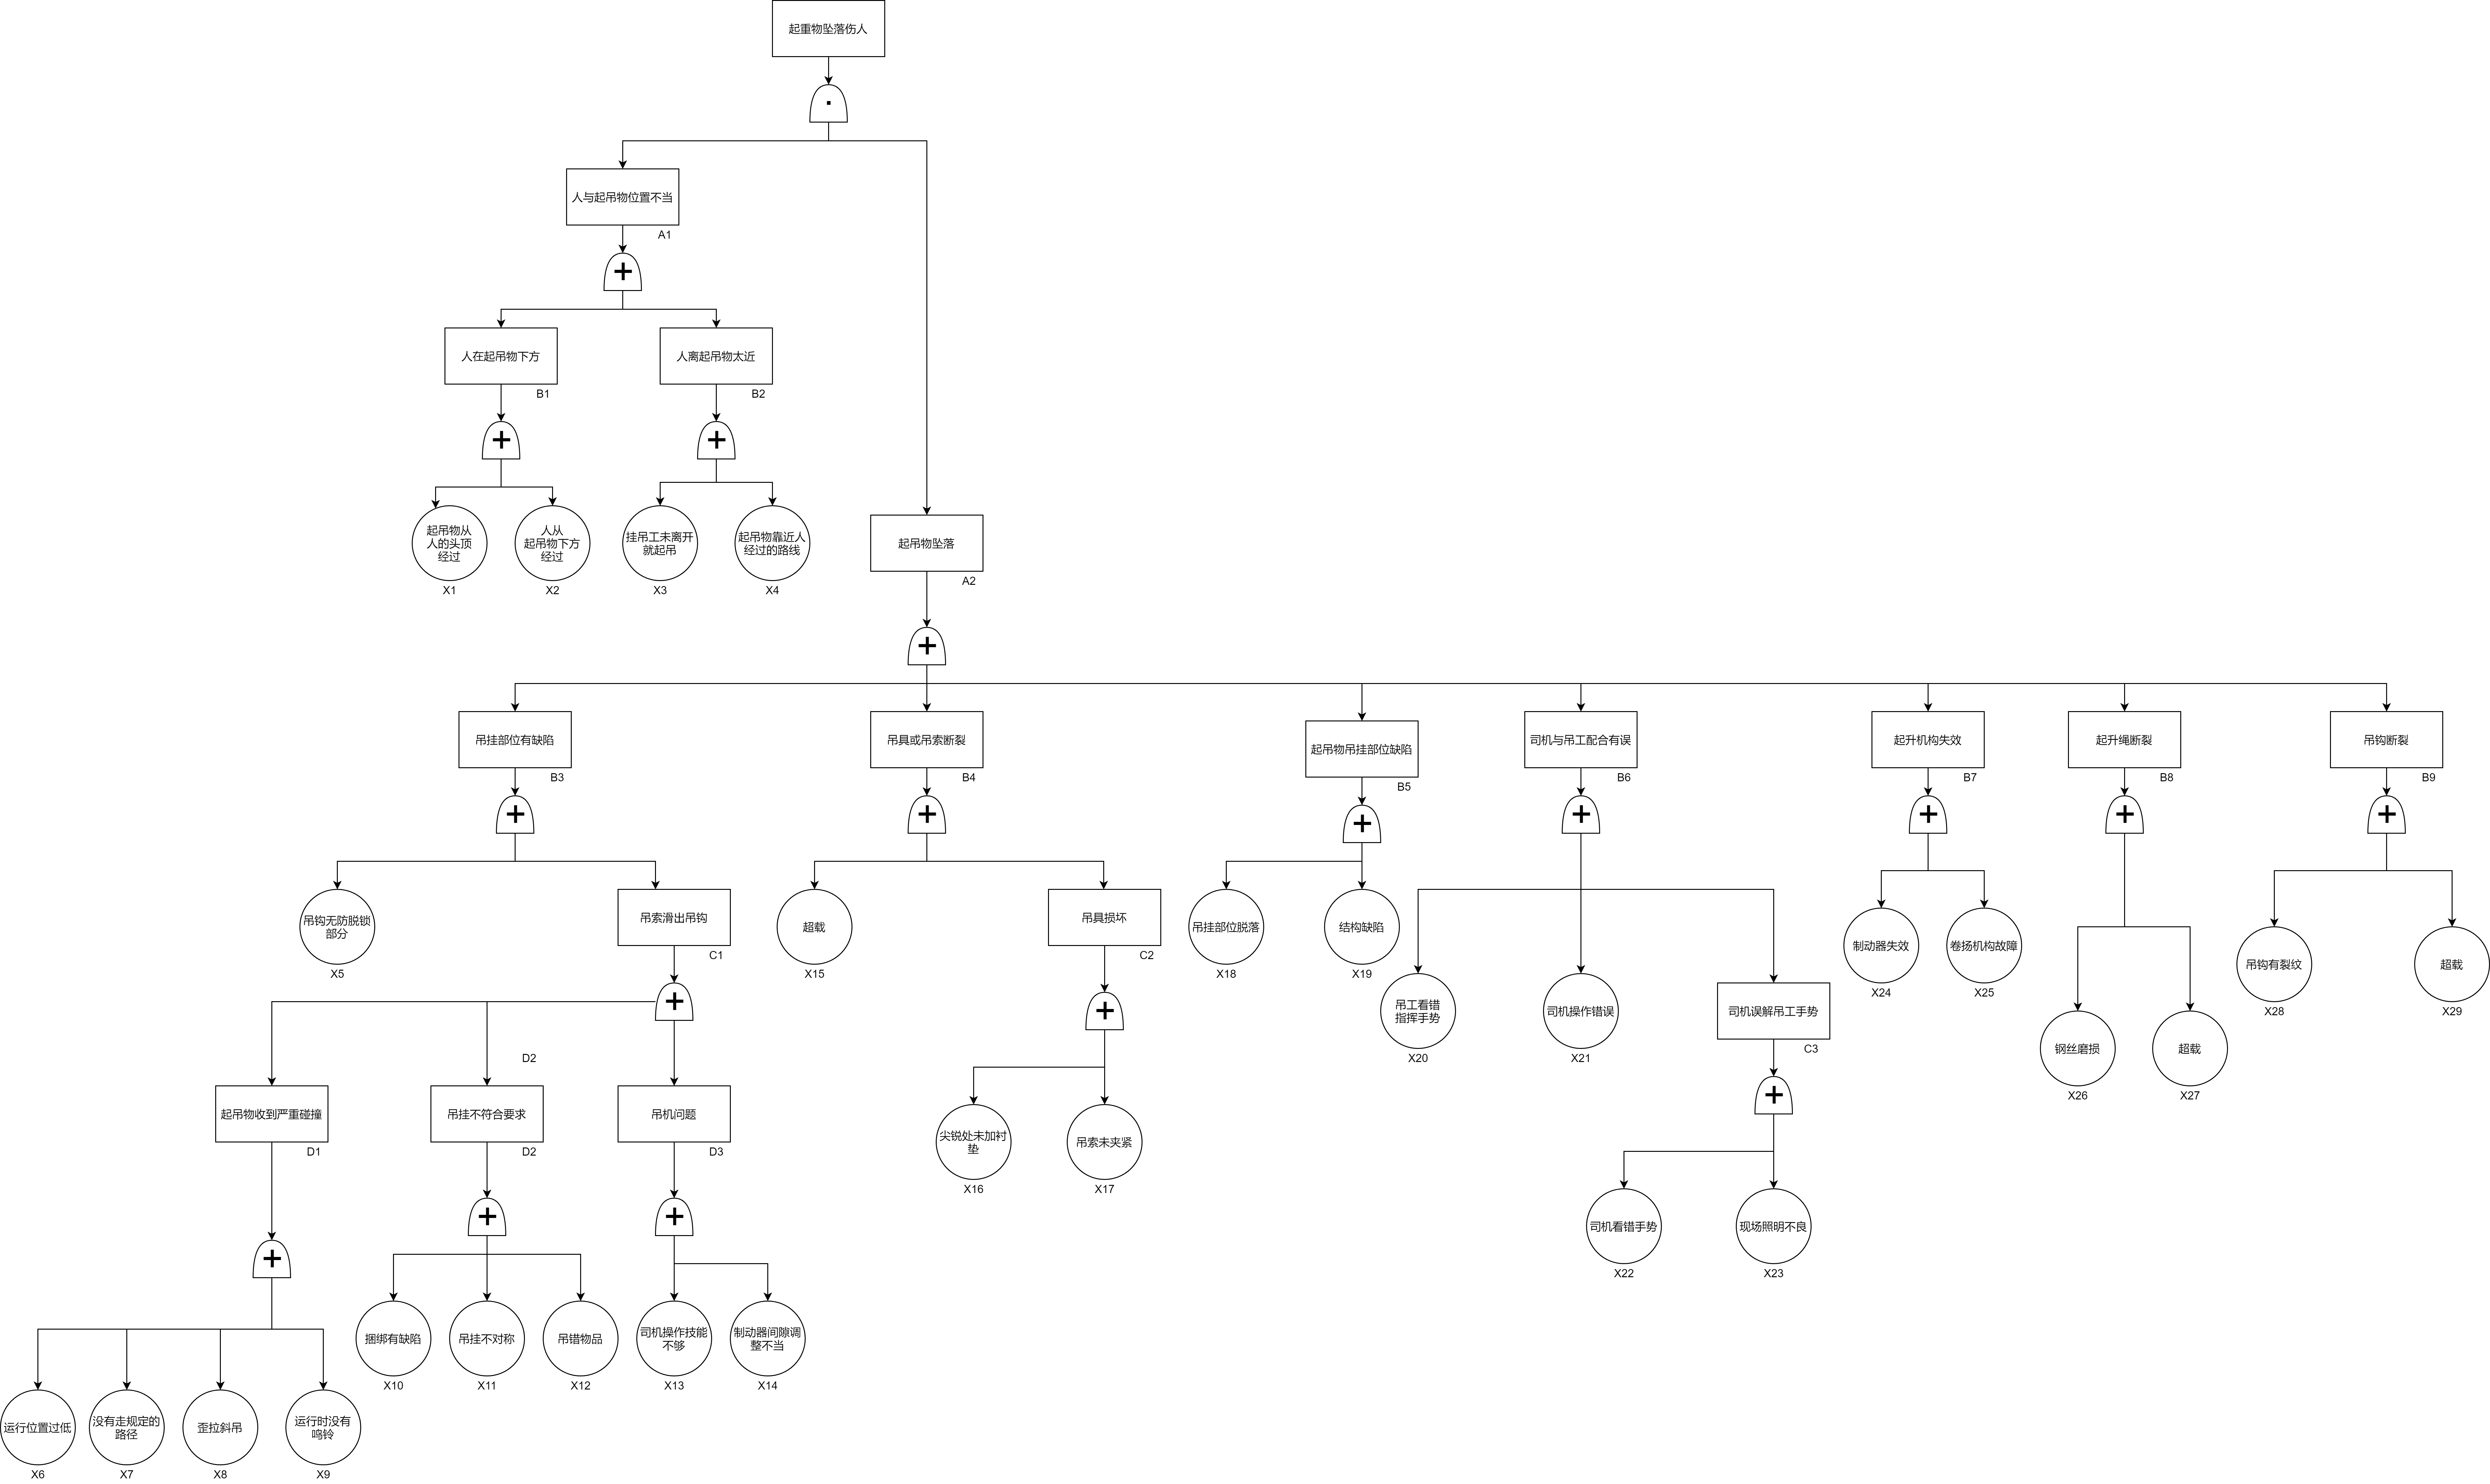
\includegraphics[width=1.0\linewidth]{figure/c3f3.png}
    \caption{吊装作业事故故障树}
    \label{fig:c3f3}
\end{figure}
\end{landscape}

在事故树中,如果所有的基本事件都发生,则顶上事件必然发生。因此,了解哪些基本事件的组合对顶上事件发生具有较大影响,这对有效地预防事故的发生是非常重要的。\\

$T=A_1A_2=(B_1+B_2)·(B_3+B_4+B_5+B_6+B_7+B_8+_B9)=[(X_1+X_2)+(X_3+X_4)]·[(X_5·C_1)+(X_{15}+C_2)+(X_{18}+X_{19})+(X_{20}+X_{21}+C_3)+(X_{24}·X_{25})+(X_{26}+X_{27})+(X_{28}+X_{29})]
=(X_1+X_2+X_3+X_4)·[X_5·(D_1+D_2+D_3)+X_{15}+(X_{16}+X_{17})+(X_{18}+X_{19})+X_{20}+X_{21}+
(X_{22}+X_{23})+X_{24}·X_{25}+X_{26}+X_{27}+X_{28}+X_{29}]
=(X_1+X_2+X_3+X_4)·[X_3·(X_6+X_7+X_8+X_9+X_{10}+X_{11}+X_{12}+X_{13}·X_{14}+X_{15}+X_{16}+X_{17}+X_{18}+X_{19}
+X_{20}+X_{21}+X_{22}+X_{23}+X_{24}+X_{25}+X_{26}+X_{27}+X_{28})]$\\

由上式求得事故树的最小割集共有 84 个,
这说明起重机械发生吊物坠落伤人的可能是非常多的。如果不采取必要的安全技术措施,这样的系统是不能被接受的。

事故树分析中的径集 G 就是系统防止事故的模式,避免顶上事件发生的最低限度的径集称最小径集。
每一个最小径集表示每一种防止顶上事件发生的途径。事故树中最小径集越多,顶上事件发生的可能性就越上,系统就越安全。\\

$T=G_1G_2G_3G_4G_5G_6G_7G_8G_9G_{10}G_{11}$\\

由上式求得该事故树的最小径集有 11 个,说明要预防起吊物坠落伤人就必须从 11 条途径进行考虑。

所以经分析,只要避免吊物从人头顶经过、避免人体从吊物下经过,避免挂吊工未离开就起吊和避免起吊物靠近人经过,就能避免起吊物伤人的发生。
预防事故要采取的措施相对要多一些。经过分析这些基本事件可分为以下四类:

(1) 第一类为起重设备及环境设施缺陷

(2) 第二类为起重设备设施的维修、保养缺陷

(3)第三类为操作人员技能缺陷

(4)第四类为违章作业

因此,只要确保起重设备、设施和工作环境完整和完好,起重司机和挂吊工培训后持证上岗,杜绝违章作业就能避免起吊物坠落,也不会发生伤人事故。


\subsubsection{吊装作业安全检查表法安全分析}

吊装作业的安全检查表的检查项目涉及有吊钩、电动机、控制盘、安全装置、钢丝绳与制动器;每一个部位都有其各自的标准和可能发生事故的频次,
具体的安全检查项目及得分情况详见表 \ref{tab:c3t1}:

\begin{landscape}
\begin{table*}[!t]
    \centering
    \caption{吊装作业的安全检查表}
    \label{tab:c3t1}
    \resizebox{240mm}{50mm}{
    \begin{tabular}{|c|c|c|c|c|c|c|c|c|c|c|c|c|c|}
    \hline
    \multirow{2}{*}{序号} & \multirow{2}{*}{检查项目} & \multirow{2}{*}{标准} & \multirow{2}{*}{不符合标准情况及后果} & \multicolumn{5}{c|}{现有控制措施} & \multicolumn{4}{c|}{风险评价} & \multirow{2}{*}{级别评价} \\ \cline{5-13}
    &  &  &  & 工程技术措施 & 管理措施 & 培训教育措施 & 个体防护措施 & 应急处置措施 & 可能性 & 严重性 & 频次 & 风险值 &  \\ \hline
   1 & 吊钩 & \begin{tabular}[c]{@{}c@{}}吊钩不得出现裂纹、磨损或者变形\\ 吊钩防脱器配置齐全。\end{tabular} & \multirow{7}{*}{起重伤害} & 设置防脱钩装置 & \begin{tabular}[c]{@{}c@{}}按照特种设备检查周期进行检查,\\ 出具检测报告\\ 有故障进行维修时,\\ 应停靠在安全地点\\ 切断电源,并\\ 挂上“禁止合闸”的警示牌\end{tabular} & \multirow{7}{*}{\begin{tabular}[c]{@{}c@{}}三级教育,\\ 每年安全培训不少于8课时;\\ 特种作业人员和维修人员持证上岗\end{tabular}} & \multirow{7}{*}{\begin{tabular}[c]{@{}c@{}}进入工作现场和上岗前,\\ 必须按岗位、工种的防护要求\\ 正确穿戴安全帽、\\ 防护手套、工作鞋、工作服。\end{tabular}} & \multirow{7}{*}{\begin{tabular}[c]{@{}c@{}}发生事故,立即进行救治\\ 如有必要拨打120就医,\\ 及时向上级汇报。\end{tabular}} & 1 & 7 & 6 & 42 & 低风险 \\ \cline{1-3} \cline{5-6} \cline{10-14} 
   2 & 电动机 & \begin{tabular}[c]{@{}c@{}}电机与联轴器连接牢固、电缆线绝缘良好;\\ 减速机无缺油、断齿\\ 固定螺栓无松动、联轴器无松动现象,\\ 减速机护罩齐全完好。\end{tabular} &  & 旋转部位设置防护罩 & \begin{tabular}[c]{@{}c@{}}按照特种设备检查周期进行检查,\\ 出具检测报告\\ 有故障进行维修时,\\ 应停靠在安全地点\\ 切断电源,并\\ 挂上“禁止合闸”的警示牌\end{tabular} &  &  &  & 3 & 2 & 6 & 36 & 低风险 \\ \cline{1-3} \cline{5-6} \cline{10-14} 
   3 & 控制盘 & \begin{tabular}[c]{@{}c@{}}控制盘固定螺栓牢固\\ 设备接地可靠\end{tabular} &  & \begin{tabular}[c]{@{}c@{}}按钮、线缆无破损\\ 设备接地良好;\\ 安全滑触线\end{tabular} & \begin{tabular}[c]{@{}c@{}}按照特种设备检查周期进行检查,\\ 出具检测报告\\ 有故障进行维修时,\\ 应停靠在安全地点\\ 切断电源,并\\ 挂上“禁止合闸”的警示牌\end{tabular} &  &  &  & 3 & 2 & 6 & 36 & 低风险 \\ \cline{1-3} \cline{5-6} \cline{10-14} 
   4 & 安全装置 & 联锁开关灵敏可靠 &  & \begin{tabular}[c]{@{}c@{}}设有联锁保护装置,\\ 限位装置\\ 极限位置缓冲装置。\end{tabular} & \begin{tabular}[c]{@{}c@{}}按照特种设备检查周期进行检查,\\ 出具检测报告\\ 有故障进行维修时,\\ 应停靠在安全地点\\ 切断电源,并\\ 挂上“禁止合闸”的警示牌\end{tabular} &  &  &  & 1 & 7 & 15 & 105 & 一般风险 \\ \cline{1-3} \cline{5-6} \cline{10-14} 
   5 & 钢丝绳 & \begin{tabular}[c]{@{}c@{}}无断丝断股现象,\\ 磨损不超标\\ 固定压板牢固,无缺油;\\ 滑轮完好可靠\end{tabular} &  & \begin{tabular}[c]{@{}c@{}}设有联锁保护装置,\\ 限位装置\\ 极限位置缓冲装置。\end{tabular} & \begin{tabular}[c]{@{}c@{}}检查钢丝绳\\ 吊钩发现失效立即更换或处理\end{tabular} &  &  &  & 3 & 2 & 6 & 36 & 低风险 \\ \cline{1-3} \cline{5-6} \cline{10-14} 
   6 & 制动器 & \begin{tabular}[c]{@{}c@{}}制动轮无裂纹\\ 制动力矩符合要求\end{tabular} &  & \begin{tabular}[c]{@{}c@{}}设有联锁保护装置,\\ 限位装置\\ 极限位置缓冲装置。\end{tabular} & \begin{tabular}[c]{@{}c@{}}检查钢丝绳\\ 吊钩发现失效立即更换或处理\end{tabular} &  &  &  & 3 & 2 & 6 & 36 & 低风险 \\ \cline{1-3} \cline{5-6} \cline{10-14} 
   7 & 导轨与滑轨 & 螺栓松动 &  & 螺栓采用防松弹垫 & 每季度检查导轨连接块松动情况和螺栓紧固情况 &  &  &  & 1 & 7 & 6 & 42 & 低风险 \\ \hline
    \end{tabular}}
    \end{table*}
\end{landscape}

\subsubsection{现场用电预先危害分析法安全分析}

现场的用电情况分为施工用变配电和一般性供电设施,对于施工用变配电的潜在危险是火灾与短路、跳闸和触电;对于一般性供电设施的潜在危险有触电和物体打击,
针对施工用变配电的火灾潜在风险做预先危害分析:\\

(1) 分析对象或系统:\\

施工用变配电\\

(2) 潜在事故:\\

火灾\\

(3) 触发事件:\\

\quan{1} 电气线路老化;

\quan{2} 电气短路;

\quan{3} 雷击;

\quan{4} 静电;

\quan{5} 变配电场所散热不良;

\quan{6} 小动物进入变配电场所;

\quan{7} 开关设备桩头松动发热;

\quan{8}小家电带至岗位使用;\\

(4) 发生条件:\\

\quan{1} 易燃、易爆物蒸气浓度达到爆炸极限 

\quan{2} 易燃物质遇明火;

\quan{3} 存在点火源、静电火花、高温物体等到引燃、引爆能量\\

(5) 事故后果:\\

人员伤亡、停产、造成严重经济损失\\

(6) 危险等级:\\

IV 灾难性的

造成人员重大伤亡及系统严重破坏的灾难性事故,必须立即予以排除\\

(7) 防范措施:\\

控制与消除火源:\\

\quan{1} 严禁吸烟、携带火种、穿带钉皮鞋进入易燃、易爆区;

\quan{2} 动火必须严格按动火手续办理动火证,并采取有效防范措施;

\quan{3} 易燃易爆场所使用防爆型电器;

\quan{4} 使用“防爆”工具,严禁钢质工具敲打、撞击、抛掷;

\quan{5} 按规定安装避雷装置,并定期进行检测;

\quan{6} 按规定采取防静电措施;\\

严格控制设备质量及其安装:\\

\quan{1} 管道、压力容器及其仪器等有关设施要按要求进行定期检验、检测、试压;

\quan{2} 对设备、管线、泵、阀、仪表、报警器、监测装置等要定期进行检查、保养、维修,保持完好状态;

\quan{3} 按标准安装电气线路,定期进行检查、维修、保养,保持完好状态;

\quan{4} 有易燃易爆物质挥发或散落的场所,高温部件要采取隔热、密闭措施;

\quan{5} 生产装置区的地沟进出口设置阻火、隔油井。\\

防止易燃、易爆物料的跑、冒、滴、漏\\

加强管理、严格工艺纪律:\\

\quan{1} 禁火区内张贴作业场所危险化学品安全标签;

\quan{2} 杜绝“三违”现象;

\quan{3} 检查有否违章、违纪现象;

\quan{4} 加强培训、教育、考核工作;

\quan{5} 防止车辆撞坏管线及管架桥等设施。\\

安全设施要齐全完好

\quan{1} 安全设施(如消防设施、遥控装置)齐全并保持完好;

\quan{2} 贮槽安装高、低液位报警器;

\quan{3}易燃、易爆场所安装可燃气体检测报警装置。\\

针对电气设备的短路跳闸潜在风险做预先危害分析:\\

(1) 分析对象或系统:\\

电气设备\\

(2) 潜在事故:\\

短路跳闸\\

(3) 触发事件:\\

\quan{1} 保护失灵或保护不当;

\quan{2} 过载;

\quan{3} 受潮;

\quan{4} 小动物;

\quan{5} 雷击;\\

(4) 发生条件:\\

\quan{1} 冲洗设备;

\quan{2} 小动物进入变配电场所;

\quan{3} 机械损伤(如动土作业、车辆振压)。\\


(5) 事故后果:\\

影响生产,引起爆炸、泄露、中毒、设备损坏等\\

(6) 危险等级:\\

III 危险的

会造成人员伤亡和系统损坏,要立即采取防范措施\\

(7) 防范措施:\\

\quan{1} 输电线路主管领导应高度重视线路跳闸故障,应根据不同季节的气候特点,及时制定线路的定期巡视和特殊巡视制度,
并认真执行。所制定的制度要任务明确,责任到人。运行人员若发现绝缘子破损、裂纹、有放电痕迹、有鸟窝或导线上挂有异物,要及时报告并排除; 

\quan{2} 运行单位要认真研究和分析线路故障的原因和特点,从中吸取教训,并在本系统内经常开展安全大检查活动,
提高各级人员的安全意识;

\quan{3} 结合春、秋检工作,并健全定期清扫、巡视制度,保证清扫、巡视责任制的落实;

\quan{4} 在鸟害集结和大风季节,要加强对线路的巡视,并在横担上安装各类防鸟装置,确保线路安全可靠运行。

\subsubsection{运输工程工作危害分析法安全分析}

在现场需要大量的水平运输以运输材料和工具。场内使用最广泛的运输工具是叉车,由于叉车作业面范围广,涉及部门复杂,极其容易包括造成误工、火灾和车辆伤害在内的诸多严重事故,
关于铲车运输的工作危害分析记录表见表 \ref{tab:c3t3}

\begin{table*}[!t]
    \centering
    \caption{运输过程中的工作危害分析记录表}
    \label{tab:c3t3}
    \resizebox{\textwidth}{!}{
        \begin{tabular}{@{}llllllll@{}}
            \toprule
            序号 & 危害 & 主要后果 & 解决方案 & L & S & 风险度 & 结论 \\ \midrule
            1 & 刹车失灵 & 车辆伤害 & 及时维修叉车同时换用手推车 & 1 & 5 & 5 & 可接受风险 \\
            2 & 方向盘失灵 & 车辆伤害 & 及时维修叉车同时换用手推车 & 1 & 5 & 5 & 可接受风险 \\
            3 & 照明不足 & 车辆伤害 & 增加照明 & 3 & 3 & 9 & 中等风险 \\
            4 & 车速过快 & 车辆伤害 & 执行铲车司机安全管理规定 & 3 & 2 & 6 & 可接受风险 \\
            5 & 铲车铲脚与地面摩擦 & 火灾 & 抬高铲脚 & 5 & 2 & 10 & 中等风险 \\
            6 & 铲角升起过高 & 车辆伤害 & 控制高度 & 3 & 2 & 6 & 可接受风险 \\
            7 & 铲车不熄火 & 车辆伤害 & 不用时熄火 & 2 & 1 & 2 & 轻微风险 \\
            8 & 铲脚不在地面 & 物体打击 & 停用时铲脚放在地面上 & 2 & 2 & 4 & 可接受风险 \\ \bottomrule
            \end{tabular}}
    \end{table*}

\subsubsection{危险区粉尘处理工作安全检查表法安全分析}

在危险区域内,粉尘的处理是一个首要问题。由于粉尘引起的火灾和爆炸不但难以避免,而且会造成巨大的人员伤亡和直接经济损失。在日常工作中,仓库,储备间等地是粉尘
集聚的高发地,产生粉尘的主要操作为搬运材料、拆装仓库等。关于粉尘处理的工作危害分析记录表见表 \ref{tab:c3t2}

\begin{table*}[!t]
    \centering
    \caption{粉尘处理的工作危害分析记录表}
    \label{tab:c3t2}
    \resizebox{\textwidth}{!}{
        \begin{tabular}{@{}ccccccccc@{}}
            \toprule
            序号 & 工作步骤 & 危害 & 主要后果 & 解决方案 & L & S & 风险度 & 结论 \\ \midrule
            1 & 搬运材料 & 仓库中存有粉尘 & 火灾或爆炸 & 作业前扫吹 & 1 & 5 & 5 & 可接受风险 \\
            2 & 搬运材料 & 负责人不在现场 & 火灾或爆炸 & 加强教育 & 2 & 5 & 10 & 中等风险 \\
            3 & 搬运材料 & 现场无消防器材 & 火灾或爆炸 & 现场常备消防器材 & 1 & 5 & 5 & 可接受风险 \\
            4 & 搬运材料 & 物料坠落 & 物体打击 & \begin{tabular}[c]{@{}c@{}}控制无关人员禁止入场\\ 佩戴安全防护用品\end{tabular} & 2 & 3 & 6 & 可接受风险 \\ \bottomrule
            \end{tabular}}
    \end{table*}
